% A short description of the experimental set-up with an image
The corresponding laboratory \textit{Aerodynamic Levitation} to the course \textit{Advanced Control Engineering 1} gives students the opportunity to model a physical system using system identification method, create the according state space model, implement a state observer, design a state-feedback controller and implement and simulate everything with MATLAB and Simulink Coder. \cite{Laborleitfaden}

The aerodynamic levitation system (figure \ref{fig:setupLevitation}) consists of a table tennis ball, a transparent hollow cylinder with a blower fan and an infrared distance sensor on the top. By controlling the speed of the blower fan, the height of the table tennis ball can be specified. Additionally, a National Instruments data acquisition card as well as a fan speed control system in combination with laboratory power supplies are used for this laboratory. \cite{Laborleitfaden}

\FloatBarrier
\begin{figure}[ht]
	\begin{center}
		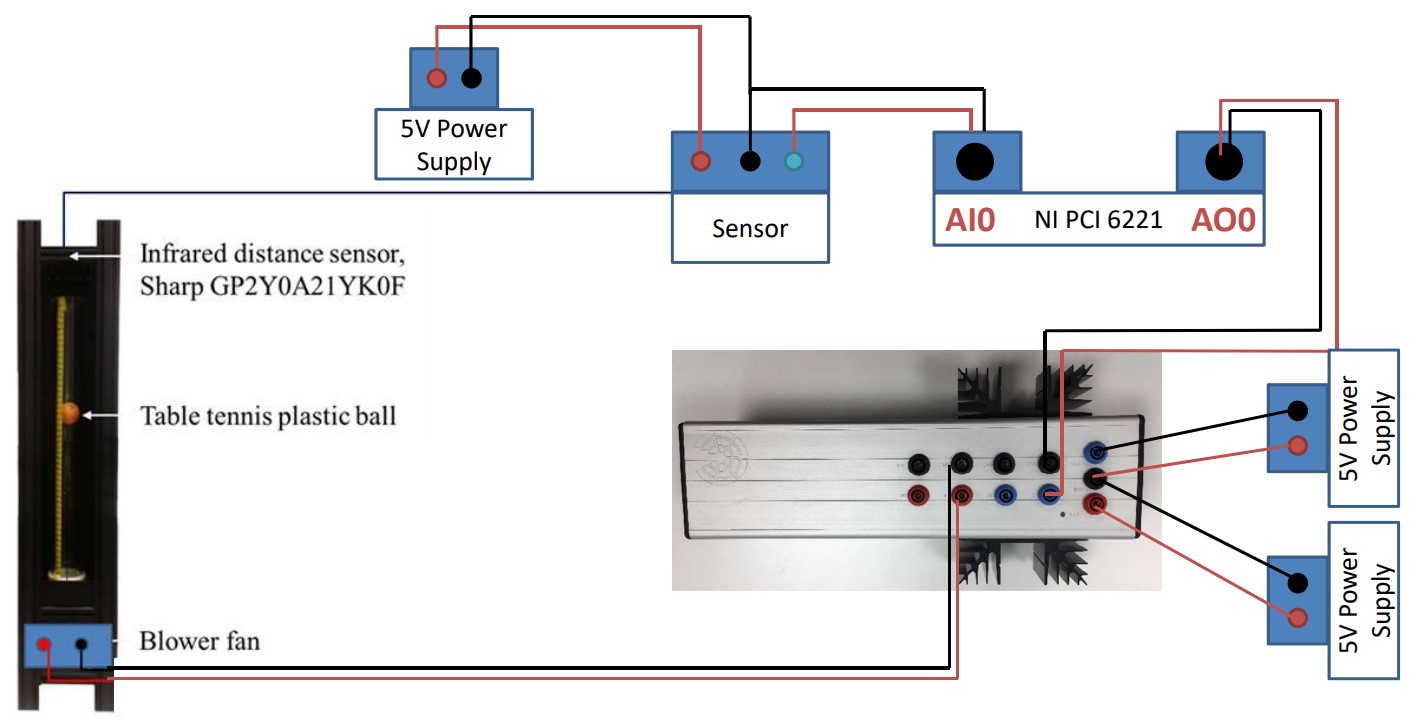
\includegraphics[width=0.7\textwidth]{figure/setupLevitation.jpg}
		\caption[Aerodynamik levitation system setup \cite{Laborleitfaden}]
                {Aerodynamik levitation system setup \cite{Laborleitfaden}}
		\label{fig:setupLevitation}
	\end{center}
\end{figure}
\FloatBarrier

The lab preparation for the first session is to fit the sensor output based on the data given on Sakai (see figure \ref{fig:fittedFunction} in the appendix \ref{appendix:firstpreparation} on page \pageref{appendix:firstpreparation}). So we get a function which computes the distance to the reflective object given in voltage to create a Simulink block which implements this conversion. Also the theory of a second-order system needs to be listed, especially the standard form in Laplace-domain, the steps required to derive the step response in the time-domain and the equation for the time-domain response for underdamped, critically damped and overdamped systems. 

In the first lab session the distance sensor gets calibrated, which means we have to take care for the signal offset as well as for the nonlinear behaviour of the sensor. To get rid of the signal offset we simply substract a contstant value from the sensor signal to get an output voltage of \SI{0}{V} when the table tennis ball was at the bottom of the cylinder. To linearize the sensor output, nine datapoints of the sensor output voltage against the distance $x$ of the table tennis ball from the sensor are taken. The values can be found in the table \ref{tab:sensor} on page \pageref{appendix:sensordata} in the appendix \ref{appendix:sensordata}. A plot of the datapoints as well as the corresponding linear function 
\begin{equation}
    f(x) = -0.0315\cdot x + 2.4758888
    \label{eqn:linearfunction }
\end{equation}
is also shown in figure \ref{fig:sensorLinearization} on page \pageref{appendix:sensordata} in the appendix \ref{appendix:sensordata}. Also during the first lab session the system identification part takes place. Therefore some step responses of the system behaviour are taken to trimm out some nice measurement data. The raw measurement data as well as the trimmed step response of the system can be seen in subfigure \ref{subfig:raw} and \ref{subfig:trimming} on page \pageref{appendix:systemidentification} in the appendix \ref{appendix:systemidentification}. Further a normalization of the system response was necessary to fit a PT2 System into the signal. The normalized signal as well as the fitted PT2 system can be seen in subfigure \ref{subfig:normalize} and \ref{subfig:fitting} on page \pageref{appendix:systemidentification} in the appendix \ref{appendix:systemidentification}.

The lab preparation for the second session consists of first creating a simulink state-space model of the PT2 system with the step response. Then an observer together with a state feedback controller can be designed in simulink with pole placement method. The whole system in simulink can be seen in figure \ref{fig:simuSimulation} in appendix \ref{appendix:secondpreparation} on page \pageref{fig:simuSimulation}. The subsystems of the \textbf{Model}, the \textbf{Controller} as well as the \textbf{Observer} are shown in figure \ref{fig:simuModel}, \ref{fig:simuController} and \ref{fig:simuObserver} in appendix \ref{appendix:secondpreparation}. In the end a step response and a challenging trajectory of the whole control system is taken from simulink. The corresponding plots are shown in figure \ref{fig:simulations} in the appendix \ref{appendix:secondpreparation} on page \pageref{fig:simulations}.

During the second and last lab session the controller is implemented on the real-world system. After the adjustments some trajectories like a sine wave are tested (appendix \ref{appendix:performance} on page \pageref{appendix:performance}).

